\documentclass[letterpaper,11pt]{article}

\usepackage[english]{babel}   
\usepackage[utf8]{inputenc}   
\usepackage{fullpage, enumerate, hyperref, graphicx}
\usepackage{fontawesome}
\pagenumbering{gobble}
\setlength\parindent{0em}
\renewcommand{\labelitemi}{$\circ$}
\newcommand{\compactlist}{\setlength{\parskip}{0pt} \setlength{\leftskip}{2em}}

\begin{document}
\begin{center}\Huge{Pablo Huijse Heise} \\ \Large{Curriculum Vitae} \end{center}



\vspace{10mm}
\begin{minipage}[t]{0.6\textwidth}
	\textbf{Name:} Pablo Andr\'es Huijse Heise \\
	\textbf{Identification number:} 16.049.102-7 \\	
	\textbf{Date of birth:} June 11, 1985  \\
	\textbf{Place of birth}: Valdivia, Chile \\
	\textbf{Marital status:} Married \\
	\textbf{Nationality:} Chilean \\
	
  
\end{minipage}
\begin{minipage}[t]{0.4\textwidth}

\centering
\vspace*{-10pt} 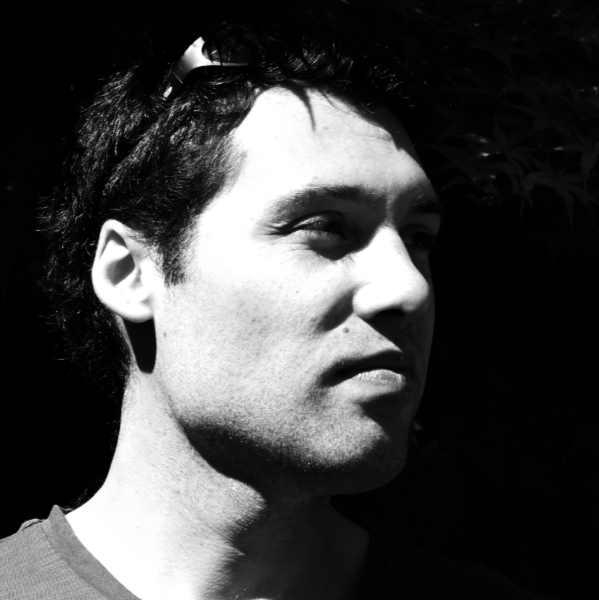
\includegraphics[scale=0.13]{../img/avatar.png}

	
\end{minipage}
	\textbf{Home Address:} Ines Gebhard Paulus 733, Villa el Bosque Sur , Valdivia, Chile \\
	\textbf{Work Address:} Instituto de Inform\'atica, Universidad Austral de Chile, General Lagos 2086, Edificio 10000, Valdivia, Chile \\
	\textbf{Contact telephone:} +56-9-98278979\\
	\textbf{Email:} phuijse (at) inf (dot) uach (dot) cl, pablo (dot) huijse (at) gmail (dot) com \\ 	
	\textbf{Website:} \url{http://phuijse.github.io} \\

\noindent\makebox[\linewidth]{\rule{\textwidth}{0.4pt}}

%\subsection*{Academic experience}
\begin{enumerate}[I]  \compactlist

	\item \textbf{Research interests} 
	
	{\leftskip 3em Astroinformatics, computational intelligence, information theory, variational methods, semi-supervised machine learning, transfer learning and active learning. High-performance computing (HPC) and general purpose graphical processing unit (GPGPU) architectures for big data problems in astronomy.\par }

	\item \textbf{Education}
		\begin{itemize} \compactlist
		\item PhD in Electrical Engineering, Universidad de Chile \hfill 2010-2014
		\begin{itemize} \compactlist
			\item Thesis title: Finding Periodicities in astronomical light curves using information theoretic learning. 
			\item Advisor: Pablo A. Est\'evez, Universidad de Chile
			\item Summary: The objective of this research is to develop robust and fully automated methods to analyse astronomical time series (light curves) in order to cope with the next generation astronomical surveys to come. The tools developed combine classical signal processing, machine learning, computational intelligence techniques and Information Theory.
		\end{itemize}
        \item Summer School in Statistics for Astronomers and Physicists XI, Penn State University \hfill 2013
		\item Electrical Engineering, Universidad de Chile \hfill 2004-2010
		\item Bachelor of Science in Electrical Engineering, Universidad de Chile \hfill 2004-2008
		\end{itemize}
	
	\item \textbf{Academic positions}
	    \begin{itemize} \compactlist
	        \item Assistant professor, Informatics Institute, Universidad Austral de Chile, Chile \hfill 2018-present
	    \end{itemize}
	
	\item \textbf{Research experience}
		\begin{itemize}  \compactlist
		\item Postdoc research ``Development of methods for big-data astronomical problems based on Information Theory and Machine Learning'', Millennium Institute of Astrophysics, Chile  \hfill2014-2017        \item Postgraduate research ``Design of an overcomplete and sparse decomposition for the correntropy function'', Computational Neuro-Engineering Laboratory, University of Florida, Gainesville, USA. Supervisor: Prof. Jos\'e C. Pr\'incipe   \hfill2013
        \item Postgraduate research ``Design of a pipeline for periodic light curve discrimination and its application to the EROS-2 database'', Institute of Applied Computational Sciences, Harvard University, Boston, USA. Supervisor: Dr. Pavlos Protopapas  \hfill2012
		\item Doctoral research ``Astronomical light curve analysis using information theoretic learning'', Universidad de Chile, Chile. Supervisor: Prof. Pablo A. Estévez \hfill2010-2014
		\item Research assistant ``Information theoretic learning functionals programmed in graphical processing units'', Universidad de Chile, Chile. Supervisor: Prof. Pablo A. Est\'evez \hfill2009
		\item Research assistant ``Robotic manipulator control and object recognition'', Universidad de Chile, Chile. Supervisor: Prof. Javier Ruiz del Solar \hfill2009
		\end{itemize}
		
	\item \textbf{Grants and scholarships}
		\begin{itemize}  \compactlist
		    \item CONICYT PAI 79170017 ``Fortalecimiento de la ciencia de datos en la Universidad Austral de Chile'' \hfill 2018-2021
		    \item FONDECYT grant N 1170305 ``Efficient methods based on information theory and machine learning for astronomical images and time series analysis'' \hfill2017-2020
			\item FONDECYT postdoctoral grant N 3150460 ``M\'etodos eficientes de procesamiento de señales basados en teoría de la información y aprendizaje de máquinas para el an\'alisis de series de tiempo astron\'omicas'' \hfill2014-2016
			\item CONICYT travel grant for doctoral students to visit the
			Computational Neuro-Engineering Laboratory at the University of Florida (7 months) \hfill2013
			\item CONICYT travel grant for doctoral students to visit the
			Institute of Applied Computational Sciences at Harvard university (8 months) \hfill2012
			\item CONICYT scholarship for PhD education in Electrical Engineering at the University
			of Chile \hfill2010-2014
		\end{itemize}
		
	
	    
	\item \textbf{Teaching experience}
	
		\begin{itemize}  \compactlist
        \item \textbf{Statistical tools for research} \\
            \textbf{Institution:} Informatics Institute, Universidad Austral de Chile, Chile \\
                \textbf{Role:} Teacher (2018-to date) \\
                \textbf{Topics:} Frequentist and Bayesian model fitting, Mixture models, MCMC
        \item \textbf{Scientific computing with Python} \\
            \textbf{Institution:} Informatics Institute, Universidad Austral de Chile, Chile \\
            \textbf{Role:} Teacher (2019) \\
            \textbf{Topics:} Python libraries for data analysis, scientific computing and HPC \\
		\item \textbf{Data mining}\\
		    \textbf{Institution:} Informatics Institute, Universidad Austral de Chile, Chile \\
            \textbf{Role:} Teacher (2018-to-date) \\
            \textbf{Topics:} Neural networks for classification, regression and feature extraction. Tensorflow, pytorch
        \item \textbf{Communications} \\
		    \textbf{Institution:} Informatics Institute, Universidad Austral de Chile, Chile \\
            \textbf{Role:} Teacher (2018-to date) \\
            \textbf{Topics:} Fourier transform, Time series analysis, Image processing
        \item \textbf{Computational Intelligence} \\
            \textbf{Institution:} Department of Electrical Engineering, Universidad de Chile, Chile \\
            \textbf{Role:} Teacher (2016-2017), Assistant teacher (2010-2013)\\
            \textbf{Topics:} Machine learning methods for classification, regression and clustering. %Neural networks, Support Vector Machines, Ensemble methods, Self-Organizing maps, K-means, Mean-Shift, Genetic Algorithms, among others. 
        \item \textbf{Neural Networks and Information Theoretic Learning} \\
            \textbf{Institution:} Department of Electrical Engineering, Universidad de Chile, Chile \\
            \textbf{Role:} Assistant teacher (2013-2015) \\
            \textbf{Topics:} Information theoretic training criteria for machine learning %, recurrent and time-delayed neural network architectures, Deep Learning, Kernel adaptive filters
        \item \textbf{INPUT-OUTPUT}, Physical Computing program, Graduate \\
            \textbf{Institution:} Universidad del Desarrollo, Chile \\
            \textbf{Role:} Responsable (2013) \\
            \textbf{Topics:} Introduction to electronics and circuit design, microcontrollers, sensors and actuators, communication and interfacing, C++ programming (Openframeworks)
 
    	\end{itemize}
        
    \item \textbf{Student supervision}
    \begin{itemize}  \compactlist{}
            
        \item Pablo Saavedra, ``Estudio de la utilizaci\'on del potencial de informaci\'on cruzado en el aprendizaje con ensamble de redes neuronales'', Department of Electrical Engineering, Universidad de Chile, 2017 (co-supervisor)
        \item Joaqu\'in Sanchez, ``An\'alisis morfol\'ogico utilizando matching pursuit para detecci\'on de husos sigma en registros polisomnogr\'aficos'', Department of Electrical Engineering, Universidad de Chile, 2016 (co-supervisor)
		\item Emanuel Berrocal, ``M\'etodos de detecci\'on de estrellas variables en im\'agenes astron\'omicas basados en factorizaci\'on no-negative de matrices'', Department of Mathematical Engineering, Universidad de Chile, 2015 (co-supervisor)
        \item Marianne Fiedler, ``Optimizaci\'on de la detecci\'on de periodos de estrellas variables en la nube de magallanes'', Universidad de los Andes, 2015 (co-supervisor)
		
		\end{itemize}
	
	
	
	\item \textbf{Publications - ISI Journals}

%\subsection*{Publications}
	\begin{itemize}  \compactlist{}
        \item \textbf{P. Huijse}, P.A. Est\'evez, F. F\"orster, S.F. Daniel, A.J. Connolly, P. Protopapas, R. Carrasco, J. C. Pr\'incipe, ``Robust period estimation using mutual information for multi-band light curves in the synoptic survey era'', \emph{The Astrophysical Journal Supplement Series}, vol. 236(1), 2018, DOI: \url{https://doi.org/10.3847/1538-4365/aab77c}
        \item R. Contreras Ramos, D. Minniti, F. Gran, M. Zocalli, J. Alonso-Garc\'ia, \textbf{P. Huijse}, M.G. Navarrio, A. Rojas-Arriagada, E. Valenti, ``The VVV Survey RR Lyrae Population in the Galactic Center Region'', \emph{The Astrophysical Journal}, vol. 863(79), DOI: \url{https://doi.org/10.3847/1538-4357/aacf90}
        \item  R. Contreras Ramos, M. Zoccali, F. Rojas, A. Rojas-Arriagada, M. G\'arate, \textbf{P. Huijse}, F. Gran, M. Soto, A. A. R. Valcarce, P.A. Es\'evez, D. Minniti, ``Proper motions in the VVV Survey: Results for more than 15 million stars across NGC 6544''', \emph{Astronomy \& Astrophysics}, vol. 608(A140), 2017, DOI: \url{https://doi.org/10.1051/0004-6361/201731462}
        \item F. F\"orster, J. C. Maureira, J. San Mart\'in, M. Hamuy, J. Mart\'inez, \textbf{P. Huijse}, G. Cabrera, L. Galbany, T. de Jaeger, S. González-Gait\'an, J. P. Anderson, H. Kuncarayakti, G. Pignata, F. Bufano, J. Litt\'in, F. Olivares, G. Medina, C. Smith, K. Vivas, P.A. Est\'evez, R. Muñoz, E. Vera, ``The High Cadence Transient Survey (HiTS) - I Survey design and supernova shock breakout constraints'', \emph{The Astrophysical Journal}, vol. 832(2), pp. 155, 2016, DOI: \url{https://doi.org/10.3847/0004-637X/832/2/155}
        \item P. Protopapas, \textbf{P. Huijse}, P.A. Estévez, P. Zegers, J. C. Príncipe, J. B. Marquette, ``A Novel, fully automated pipeline for period estimation in the {EROS}-2 Data set'', \emph{The Astrophysical Journal Supplement Series}, vol. 216(2), 2015, DOI: \url{https://doi.org/10.1088/0067-0049/216/2/25}
        \item \textbf{P. Huijse}, P. A. Estévez, P. Protopapas, J. C. Príncipe, and P. Zegers, ``Computational Intelligence Challenges and Applications on Large-Scale Astronomical Time Series Databases'', \emph{IEEE Computational Intelligence Magazine}, vol. 9(3), 2014, DOI: \url{https://doi.org/10.1109/MCI.2014.2326100}, \href{https://arxiv.org/pdf/1509.07823.pdf}{\faExternalLink}
        \item  \textbf{P. Huijse}, P.A. Estévez, P. Zegers, J. C. Príncipe, P. Protopapas, ``An Information Theoretic Algorithm for Finding Periodicities in Stellar Light Curves'', \emph{IEEE Transactions on Signal Processing}, vol. 60(10), pp. 5135-5145, 2012
        \item \textbf{P. Huijse}, P.A. Estévez, P. Zegers, J. C. Príncipe, P. Protopapas, ``Period Estimation in Astronomical Time Series Using Slotted Correntropy'', \emph{IEEE Signal Processing Letters}, vol. 18(6), pp. 371-374, 2011
	\end{itemize}


    \item \textbf{Publications - Conference Proceedings}

	\begin{itemize}  \compactlist{}
        \item  N. Astorga, \textbf{P. Huijse}, P.A. Est\'evez and F. Forster, ``Clustering of Astronomical Transient Candidates Using Deep Variational Embedding'', Proceedings of the International Joint Conference on Neural Networks (IJCNN) 2019, July 2018, \url{https://doi.org/10.1109/IJCNN.2018.8489358}            
        \item \textbf{P. Huijse}, N. Astorga, P.A. Est\'evez, G. Pignata, ``Latent representations of transient candidates from an astronomical image difference pipeline using Variational Autoencoders'', Proceedings of the European Symposium on Artificial Neural Networks (ESANN), Bruges, Belgium, 2018, ISBN 978-2-87-587047-6, \href{https://www.elen.ucl.ac.be/esann/proceedings/papers.php?ann=2018}{\faExternalLink}.
        \item S. Ulloa, P. A. Estevez, \textbf{P. Huijse}, C. M. Held, C. A. Perez, R. Chamorro, M. Garrido, C. Algarin, P. Peirano, ``Sleep-Spindle Identification on EEG Signals from Polysomnographic Recordings Using Correntropy'', 38th Annual International Conference of the IEEE Engineering in Medicine and Biology Society (EMBC), Orlando, FL, 2016, pp. 3736-3739.
        \item \textbf{P. Huijse}, P. A. Estévez, F. Förster, E. Berrocal, ``Discriminating Variable Star Candidates in Large Image Databases from the HiTS Survey Using NMF'', Procedia Computer Science, vol. 53, pp. 29-38, 2015. Presented at the INNS Conference on Big Data 2015 Program San Francisco, CA, USA, 2015
        \item D. Nova, P. A. Estévez, \textbf{P. Huijse}, ``K-Nearest Neighbor Nonnegative Matrix Factorization for Learning a Mixture of Local SOM Models'', Advances in Intelligent Systems and Computing, Part IV, vol. 295, pp. 229-238, Springer, 2014. Proceedings of the 10th International Workshop, WSOM 2014, Mittweida, Germany,  2014
        \item \textbf{P. Huijse}, P.A. Estévez, P. Protopapas, P. Zegers, J. C. Príncipe,  ``Computational Challenges in Processing Very Large Astronomical Survey Databases'', Proceeding of the 2012 9th Asia-Pacific Symposium on Information and Telecommunication Technologies (APSITT), 2012
        \item P.A. Estévez, \textbf{P. Huijse}, P. Zegers, J. C. Príncipe, P. Protopapas, ``Period Detection in Light Curves from Astronomical Objects Using Correntropy'', Proceedings of the 2010 International Joint Conference on Neural Networks (IJCNN), pp. 1-7, Barcelona,  2010
	\end{itemize}

    \item \textbf{Talks, presentations and posters}
        \begin{itemize}  \compactlist{}
        \item ``Oportunidades para científicos de datos e ingenieros en la era de big-data en astronomía'', \emph{Seminar series at UACH}, April, 2018 and 2019
        \item ``Representation learning for astronomical data using neural networks'', \emph{LSST Chile Workshop 2019}, La Serena, March, 2019
        \item ``Learning representations using Variational Autoencoders'', \emph{EVIC 2019}, Santiago, December, 2018
        \item ``Tutorial on astronomical data analysis using machine learning'', \emph{Schools on Systems and Networks 2018}, Valdivia, October, 2018
        \item ``Robust period estimation using mutual information for multi-band light curves'', \emph{CMM Pucón Symposium}, Puerto Varas, Chile, August 2017
        \item ``Information theory and semi supervised machine learning with applications in Astronomy'', \emph{Summer School on Computational Intelligence and Robotics (EVIC)}, Universidad de los Andes, Chile, December 2016
        \item ``Astronomical time series analysis using information theoretic criteria'', \emph{Astroinformatics 2016 conference}, Sorrento, Italy, October 2016
        \item ``Machine learning classification of multi-band supernovae light curves'', \emph{Supernovae through the Ages conference}, Easter Island, Chile, August 2016
        \item ``Semi-supervised classification of HiTS candidates using active learning'', \emph{Pucón Symposium}, Puerto Varas, Chile, August 2015
        \item ``Using information theoretic tools and GPGPU to mine periodic variable stars from the EROS-2 survey'', \emph{NOAO: Tools for Astronomical Big Data workshop}, Tucson, USA, March 2015
        \item ``Time-frequency analysis using information theory and non-negative matrix factorization'', \emph{Summer School on Computational Intelligence and Robotics (EVIC)}, Universidad de Chile, Chile, December 2014
        \item ``A high resolution periodogram using correntropy and non-negative matrix Factorization'', \emph{Astroinformatics 2014 conference}, Valparaiso, Chile, August 2014
        \item ``Mining periodic variable stars in astronomical light curve Ddatabases using information theoretic criteria'', \emph{The 5th VVV meeting}, Concon, Chile, April 2014
        \item ``Finding periodicities in astronomical light curves using information theoretic learning'', \emph{Digging deeper and faster: algorithms for computationally limited problems in time-domain astronomy}, Caltech, Pasadena, USA, December 2011
        \end{itemize}
        
	\item \textbf{Technical skills}
		\begin{itemize} \compactlist
			\item \textbf{Programming languages:} Proficient in C, C++,  Python and Cython, experienced with C\#, CUDA, OpenMP and GNU bash, familiar with R, basic knowledge of Javascript, Verilog, SQL, GTK+ and QT
			\item \textbf{Operating systems and platforms:} Proficient with GNU Linux, Arduino/AVR, Raspberry PI, Olimexino and Teensy (ARM), experienced with MS Windows 
			\item \textbf{Software:} Proficient with Matlab, Unity, Openframeworks, Blender, familiar with Processing
			\item \textbf{Publishing:} Experienced with Latex, Beamer and Inkscape
		\end{itemize}
        
	
	\item \textbf{Languages} 
	
	{\leftskip 3em  Spanish (native), English (fluent). \par }
	
	%\newpage
	
%	\item \textbf{Outside academia}
%		\begin{itemize}  \compactlist
%		\item Founder of Qualia \hfill2011-today \\
%		In Qualia we use electronics and computational tools to develop interfaces to approximate our physical bodies to the virtual world. We focus on applications related with music and the learning processes associated to it. More information at \url{http://www.qualiastudio.cl/}
%		\end{itemize}
		
	\item \textbf{Other interests} 
	
	{\leftskip 3em Interactive design, 3D printing, augmented reality, physical interfaces, music synthesis, generative art and computational creativity,  fractals, embedded systems, video game design and game engines, karate-do, transverse flute and saxophone, cooking, japanese animation and culture, hiking.  \par }

	
\end{enumerate}


\end{document}
